\chapter{结果与讨论}

\section{润滑体系研究}

\subsection{配方设计}
本实验中使用了 1 种聚乙烯蜡:PEW-0380 以及 3 种氧化聚乙烯蜡:AC-316、AC-617、AC-629。聚乙烯蜡为乙烯的低度聚合产品,具有良好的中期及后期润滑性,并能在 CPVC 注塑加工中作为脱模剂使用。氧化聚乙烯蜡为含羧基的低分子量聚乙烯,并含有醇、酮及酯类化合物。由于氧化使烷烃链上生成一定数量极性的羧基,提高了它在 CPVC 的相容性,使其同时兼有良好的内、外润滑性能,并赋予制品良好的透明性和光泽性。\par
一般认为,外润滑剂的加入会使材料的力学和耐热性能均有所下降。因此我们通过控制其他组成不变,单独改变外润滑剂的种类,从而找到一种在相同用量下能实现最好润滑效果且对材料热稳定性和力学性能影响最小的外润滑剂种类。具体配方如表 \ref{tab1Pre} 所示。

\begin{table}[!htb]
    \caption{CPVC 4 种外润滑剂配方设计表}
    \label{tab1Pre}
    \begin{center}
    \footnotesize{
        \begin{tabular}{ccccccccccc}
            \borderLine
            组别 & CPVC & \makecell[c]{抗冲击\\改性剂} & 有机锡 & \makecell[c]{AC-\\316} & \makecell[c]{AC-\\617} & \makecell[c]{AC-\\629} & \makecell[c]{PEW-\\0380} & \makecell[c]{汉高\\G-60} & \makecell[c]{加工\\助剂} & \makecell[c]{钛白粉}   \\
            \interLine
            $E_1$ & 100 & 8 & 2 & 1.3 & & & & 1.2 & 3 & 2   \\
            $E_2$ & 100 & 8 & 2 & & 1.3 & & & 1.2 & 3 & 2   \\
            $E_3$ & 100 & 8 & 2 & & & 1.3 & & 1.2 & 3 & 2   \\
            $E_4$ & 100 & 8 & 2 & & & & 1.3 & 1.2 & 3 & 2   \\
            \borderLine
        \end{tabular}
    }
    \end{center}
\end{table}

\subsection{热老化试验箱法}

将 4 组配方的样板进行切割,取 1 $\rm{cm^2}$ 的试样进行测试,结果如表 \ref{tab1static} 所示。

\begin{table}[!htb]
    \caption{$E_1 \sim E_4$ 组热老化试验箱法样品颜色随时间变化}
    \label{tab1static}
    \begin{center}
    \footnotesize{
        \begin{tabular}{cccccccc}
            \borderLine
            \multirow{2}{*}{Sample} & \multicolumn{7}{c}{加入不同种类润滑剂的 CPVC 试样 180\cd 烘箱中颜色随时间的变化}\\
            \cline{2-8}
            & 0 min & 20 min & 30 min & 70 min & 120 min & 250 min & 360 min  \\
            \interLine 
            $E_1$ & \makecell[c]{
\includegraphics[width=.1\linewidth]{src/origin/1/static/00.png}} & \makecell[c]{
\includegraphics[width=.1\linewidth]{src/origin/1/static/01.png}} & \makecell[c]{
\includegraphics[width=.1\linewidth]{src/origin/1/static/02.png}} & \makecell[c]{
\includegraphics[width=.1\linewidth]{src/origin/1/static/03.png}} & \makecell[c]{
\includegraphics[width=.1\linewidth]{src/origin/1/static/04.png}} & \makecell[c]{
\includegraphics[width=.1\linewidth]{src/origin/1/static/05.png}} & \makecell[c]{
\includegraphics[width=.1\linewidth]{src/origin/1/static/06.png}}   \\
            $E_2$ & \makecell[c]{
\includegraphics[width=.1\linewidth]{src/origin/1/static/10.png}} & \makecell[c]{
\includegraphics[width=.1\linewidth]{src/origin/1/static/11.png}} & \makecell[c]{
\includegraphics[width=.1\linewidth]{src/origin/1/static/12.png}} & \makecell[c]{
\includegraphics[width=.1\linewidth]{src/origin/1/static/13.png}} & \makecell[c]{
\includegraphics[width=.1\linewidth]{src/origin/1/static/14.png}} & \makecell[c]{
\includegraphics[width=.1\linewidth]{src/origin/1/static/15.png}} & \makecell[c]{
\includegraphics[width=.1\linewidth]{src/origin/1/static/16.png}}  \\
            $E_3$ & \makecell[c]{
\includegraphics[width=.1\linewidth]{src/origin/1/static/20.png}} & \makecell[c]{
\includegraphics[width=.1\linewidth]{src/origin/1/static/21.png}} & \makecell[c]{
\includegraphics[width=.1\linewidth]{src/origin/1/static/22.png}} & \makecell[c]{
\includegraphics[width=.1\linewidth]{src/origin/1/static/23.png}} & \makecell[c]{
\includegraphics[width=.1\linewidth]{src/origin/1/static/24.png}} & \makecell[c]{
\includegraphics[width=.1\linewidth]{src/origin/1/static/25.png}} & \makecell[c]{
\includegraphics[width=.1\linewidth]{src/origin/1/static/26.png}}  \\
            $E_4$ & \makecell[c]{
\includegraphics[width=.1\linewidth]{src/origin/1/static/30.png}} & \makecell[c]{
\includegraphics[width=.1\linewidth]{src/origin/1/static/31.png}} & \makecell[c]{
\includegraphics[width=.1\linewidth]{src/origin/1/static/32.png}} & \makecell[c]{
\includegraphics[width=.1\linewidth]{src/origin/1/static/33.png}} & \makecell[c]{
\includegraphics[width=.1\linewidth]{src/origin/1/static/34.png}} & \makecell[c]{
\includegraphics[width=.1\linewidth]{src/origin/1/static/35.png}} & \makecell[c]{
\includegraphics[width=.1\linewidth]{src/origin/1/static/36.png}}    \\
            \borderLine
        \end{tabular}
    }
    \end{center}
\end{table}

从表 \ref{tab1static} 可以看出,$E_1$ 组和 $E_2$ 组的样品在实验开始的 20 min 后表面开始出现起伏,当 360 min 时,其表面已严重变黑且因 CPVC 分解产生 HCl 而形成了大量的气泡。说明 AC-316 与 AC-617 对 CPVC 树脂的塑化效果改善不大,CPVC 树脂由于塑化不佳致其容易发生分解。$E_4$ 组在 360 min 时轻微发黄,认为 PEW-0380 对 CPVC 塑化效果改善最大。

\subsection{动态热稳定性测试}

图 \ref{fig1Hakee} 所示为 $E_1 \sim E_4$ 四种配方在转矩流变仪中进行加热剪切过程的 转矩-时间 曲线。由图中数据可得到该体系的熔化转矩、平衡转矩与热稳定时间\footnote{见 \pageref{sectionHakee} 页 \ref{sectionHakee} 动态热稳定性},具体数据见表 \ref{tab1Hakee}所示。

\begin{figure}[!htb]
    \begin{center}
        % GNUPLOT: LaTeX picture with Postscript
\begingroup
  \makeatletter
  \providecommand\color[2][]{%
    \GenericError{(gnuplot) \space\space\space\@spaces}{%
      Package color not loaded in conjunction with
      terminal option `colourtext'%
    }{See the gnuplot documentation for explanation.%
    }{Either use 'blacktext' in gnuplot or load the package
      color.sty in LaTeX.}%
    \renewcommand\color[2][]{}%
  }%
  \providecommand\includegraphics[2][]{%
    \GenericError{(gnuplot) \space\space\space\@spaces}{%
      Package graphicx or graphics not loaded%
    }{See the gnuplot documentation for explanation.%
    }{The gnuplot epslatex terminal needs graphicx.sty or graphics.sty.}%
    \renewcommand\includegraphics[2][]{}%
  }%
  \providecommand\rotatebox[2]{#2}%
  \@ifundefined{ifGPcolor}{%
    \newif\ifGPcolor
    \GPcolorfalse
  }{}%
  \@ifundefined{ifGPblacktext}{%
    \newif\ifGPblacktext
    \GPblacktexttrue
  }{}%
  % define a \g@addto@macro without @ in the name:
  \let\gplgaddtomacro\g@addto@macro
  % define empty templates for all commands taking text:
  \gdef\gplbacktext{}%
  \gdef\gplfronttext{}%
  \makeatother
  \ifGPblacktext
    % no textcolor at all
    \def\colorrgb#1{}%
    \def\colorgray#1{}%
  \else
    % gray or color?
    \ifGPcolor
      \def\colorrgb#1{\color[rgb]{#1}}%
      \def\colorgray#1{\color[gray]{#1}}%
      \expandafter\def\csname LTw\endcsname{\color{white}}%
      \expandafter\def\csname LTb\endcsname{\color{black}}%
      \expandafter\def\csname LTa\endcsname{\color{black}}%
      \expandafter\def\csname LT0\endcsname{\color[rgb]{1,0,0}}%
      \expandafter\def\csname LT1\endcsname{\color[rgb]{0,1,0}}%
      \expandafter\def\csname LT2\endcsname{\color[rgb]{0,0,1}}%
      \expandafter\def\csname LT3\endcsname{\color[rgb]{1,0,1}}%
      \expandafter\def\csname LT4\endcsname{\color[rgb]{0,1,1}}%
      \expandafter\def\csname LT5\endcsname{\color[rgb]{1,1,0}}%
      \expandafter\def\csname LT6\endcsname{\color[rgb]{0,0,0}}%
      \expandafter\def\csname LT7\endcsname{\color[rgb]{1,0.3,0}}%
      \expandafter\def\csname LT8\endcsname{\color[rgb]{0.5,0.5,0.5}}%
    \else
      % gray
      \def\colorrgb#1{\color{black}}%
      \def\colorgray#1{\color[gray]{#1}}%
      \expandafter\def\csname LTw\endcsname{\color{white}}%
      \expandafter\def\csname LTb\endcsname{\color{black}}%
      \expandafter\def\csname LTa\endcsname{\color{black}}%
      \expandafter\def\csname LT0\endcsname{\color{black}}%
      \expandafter\def\csname LT1\endcsname{\color{black}}%
      \expandafter\def\csname LT2\endcsname{\color{black}}%
      \expandafter\def\csname LT3\endcsname{\color{black}}%
      \expandafter\def\csname LT4\endcsname{\color{black}}%
      \expandafter\def\csname LT5\endcsname{\color{black}}%
      \expandafter\def\csname LT6\endcsname{\color{black}}%
      \expandafter\def\csname LT7\endcsname{\color{black}}%
      \expandafter\def\csname LT8\endcsname{\color{black}}%
    \fi
  \fi
    \setlength{\unitlength}{0.0500bp}%
    \ifx\gptboxheight\undefined%
      \newlength{\gptboxheight}%
      \newlength{\gptboxwidth}%
      \newsavebox{\gptboxtext}%
    \fi%
    \setlength{\fboxrule}{0.5pt}%
    \setlength{\fboxsep}{1pt}%
\begin{picture}(7200.00,5040.00)%
    \gplgaddtomacro\gplbacktext{%
      \csname LTb\endcsname%
      \put(814,704){\makebox(0,0)[r]{\strut{}$-10$}}%
      \put(814,1213){\makebox(0,0)[r]{\strut{}$-5$}}%
      \put(814,1722){\makebox(0,0)[r]{\strut{}$0$}}%
      \put(814,2231){\makebox(0,0)[r]{\strut{}$5$}}%
      \put(814,2740){\makebox(0,0)[r]{\strut{}$10$}}%
      \put(814,3248){\makebox(0,0)[r]{\strut{}$15$}}%
      \put(814,3757){\makebox(0,0)[r]{\strut{}$20$}}%
      \put(814,4266){\makebox(0,0)[r]{\strut{}$25$}}%
      \put(814,4775){\makebox(0,0)[r]{\strut{}$30$}}%
      \put(946,484){\makebox(0,0){\strut{}$0$}}%
      \put(1678,484){\makebox(0,0){\strut{}$1$}}%
      \put(2410,484){\makebox(0,0){\strut{}$2$}}%
      \put(3142,484){\makebox(0,0){\strut{}$3$}}%
      \put(3875,484){\makebox(0,0){\strut{}$4$}}%
      \put(4607,484){\makebox(0,0){\strut{}$5$}}%
      \put(5339,484){\makebox(0,0){\strut{}$6$}}%
      \put(6071,484){\makebox(0,0){\strut{}$7$}}%
      \put(6803,484){\makebox(0,0){\strut{}$8$}}%
    }%
    \gplgaddtomacro\gplfronttext{%
      \csname LTb\endcsname%
      \put(176,2739){\rotatebox{-270}{\makebox(0,0){\strut{}转矩/N$\cdot$m}}}%
      \put(3874,154){\makebox(0,0){\strut{}时间/min}}%
      \csname LTb\endcsname%
      \put(5816,1537){\makebox(0,0)[r]{\strut{}AC-316}}%
      \csname LTb\endcsname%
      \put(5816,1317){\makebox(0,0)[r]{\strut{}AC-617}}%
      \csname LTb\endcsname%
      \put(5816,1097){\makebox(0,0)[r]{\strut{}AC-629}}%
      \csname LTb\endcsname%
      \put(5816,877){\makebox(0,0)[r]{\strut{}PEW-0380}}%
    }%
    \gplbacktext
    \put(0,0){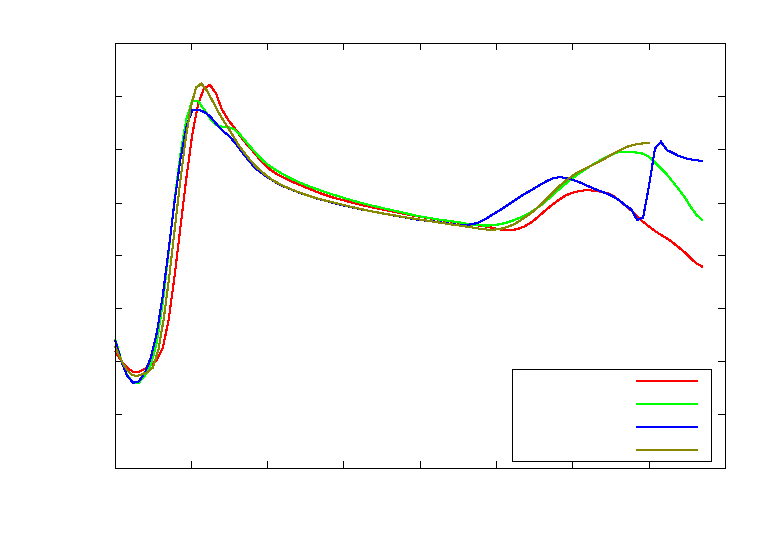
\includegraphics{src/origin/1/hakee}}%
    \gplfronttext
  \end{picture}%
\endgroup

    \end{center}
    \caption{$E_1 \sim E_4$ 组转矩流变仪 转矩-时间 曲线}
    \label{fig1Hakee}
\end{figure}

\begin{table}[!htb]
    \caption{$E_1 \sim E_4$ 组动态热稳定性能数据表}
    \label{tab1Hakee}
    \begin{center}
    \footnotesize{
        \begin{tabular}{ccccc}
            \borderLine
            组别 & 润滑剂种类 & \makecell[c]{熔化转矩 $M_{fus}$/\\N$\cdot$m} & \makecell[c]{平衡转矩$M_{melt}$/\\N$\cdot$m} & \makecell[c]{热稳定时间$T_{s}$/\\min} \\
            \interLine
            $E_1$ & AC-316 & 29.6 & 12.1 & 6.2  \\
            $E_2$ & AC-617 & 26.5 & 12.5 & 6.6  \\
            $E_3$ & AC-629 & 24.9 & 12.4 & 5.9  \\
            $E_4$ & PEW-0380 & 28.0 & 12.2 & 7.3    \\
            \borderLine
        \end{tabular}
    }
    \end{center}
\end{table}

结合图表数据可以看出,将试样加入到转矩流变仪后,$E_2$ 组和 $E_3$ 组的熔化转矩明显小于 $E_1$ 组和 $E_4$ 组,认为 $E_2$ 组和 $E_3$ 组的混合物熔体黏度小于 $E_1$ 组和 $E_4$ 组。考虑到 4 种外润滑剂的黏度相差较大,分析是 AC-316 和 PEW-0380 的黏度较 AC-617 和 AC-629 的大,因此在熔化初期其在 CPVC 熔体表面的分布不佳,导致熔化转矩相对较高。随着时间的进行,$E_2$ 组和 $E_3$ 组首先到达平衡转矩的最低点,并且该其平衡转矩略大于 $E_1$ 组和 $E_4$ 组,因此认为在长时间的塑化过程中,AC-316 与 PEW-0380 仍能保持较好的润滑效果,原因为 AC-617 与 AC-629 的滴点较 AC-316 与 PEW-0380 更低,因此在塑化加工过程中,温度逐渐上升,AC-617 与 AC-629 首先失效 导致其平衡转矩较大,加工性能变差。$E_4$ 组具有最长的热稳定时间,其 $T_{s}$ 为 7.3 min,能够满足 CPVC 塑化加工的要求。

\subsection{力学性能测试}

采用万能试验机对 $E_1 \sim E_4$ 组的标准试样进行拉伸强度、弯曲强度和缺口冲击强度的测试,具体数据如表 \ref{tab1Mach} 所示。

\begin{table}[!htb]
    \caption{$E_1 \sim E_4$ 组力学性能数据表}
    \label{tab1Mach}
    \begin{center}
    \footnotesize{
        \begin{tabular}{cccc}
			\borderLine
			组别 & \makecell[c]{拉伸强度$\sigma_t$/\\MPa} & \makecell[c]{弯曲强度$\sigma_{b}$/\\Mpa} & \makecell[c]{缺口冲击强度$aiN$/\\$\rm{KJ/m^2}$}\\
			\interLine
			$E_1$ & 57.30 & 63.73 & 8.01	\\
			$E_2$ & 59.16 & 60.29 & 10.57	\\
			$E_3$ & 58.77 & 60.59 & 14.10	\\
			$E_4$ & 59.48 & 60.61 & 16.04	\\
			\borderLine
        \end{tabular}
    }
    \end{center}
\end{table}

从表中数据可见,四组的拉伸强度和弯曲强度差别不大,但缺口冲击强度呈 $aiN_{E_4} > aiN_{E_3} > aiN_{E_2} > aiN_{E_1}$ 的趋势,并且 $E_4$ 组的缺口冲击强度远好于 $E_1$ 组 和 $E_2$ 组。分析原因为 PEW-0380 在 CPVC 的塑化过程中,能够保持较好的润滑作用,使得 CPVC 分子在较少发生热分解的情况下部分断裂生成分子量较小的 CPVC 链,从而实现较好的塑化效果。这部分较短的 CPVC 分子链为体系提供了很大的冲击强度以及韧性的改善。

\subsection{动态力学热分析(DMA)}

根据 $E_1 \sim E_4$ 四组配方的 损耗因子-时间 数据制得图 \ref{fig1Tg},取损耗因子的峰值温度作为试样的玻璃化转变温度。

\begin{figure}[!htb]
    \begin{center}
        % GNUPLOT: LaTeX picture with Postscript
\begingroup
  \makeatletter
  \providecommand\color[2][]{%
    \GenericError{(gnuplot) \space\space\space\@spaces}{%
      Package color not loaded in conjunction with
      terminal option `colourtext'%
    }{See the gnuplot documentation for explanation.%
    }{Either use 'blacktext' in gnuplot or load the package
      color.sty in LaTeX.}%
    \renewcommand\color[2][]{}%
  }%
  \providecommand\includegraphics[2][]{%
    \GenericError{(gnuplot) \space\space\space\@spaces}{%
      Package graphicx or graphics not loaded%
    }{See the gnuplot documentation for explanation.%
    }{The gnuplot epslatex terminal needs graphicx.sty or graphics.sty.}%
    \renewcommand\includegraphics[2][]{}%
  }%
  \providecommand\rotatebox[2]{#2}%
  \@ifundefined{ifGPcolor}{%
    \newif\ifGPcolor
    \GPcolorfalse
  }{}%
  \@ifundefined{ifGPblacktext}{%
    \newif\ifGPblacktext
    \GPblacktexttrue
  }{}%
  % define a \g@addto@macro without @ in the name:
  \let\gplgaddtomacro\g@addto@macro
  % define empty templates for all commands taking text:
  \gdef\gplbacktext{}%
  \gdef\gplfronttext{}%
  \makeatother
  \ifGPblacktext
    % no textcolor at all
    \def\colorrgb#1{}%
    \def\colorgray#1{}%
  \else
    % gray or color?
    \ifGPcolor
      \def\colorrgb#1{\color[rgb]{#1}}%
      \def\colorgray#1{\color[gray]{#1}}%
      \expandafter\def\csname LTw\endcsname{\color{white}}%
      \expandafter\def\csname LTb\endcsname{\color{black}}%
      \expandafter\def\csname LTa\endcsname{\color{black}}%
      \expandafter\def\csname LT0\endcsname{\color[rgb]{1,0,0}}%
      \expandafter\def\csname LT1\endcsname{\color[rgb]{0,1,0}}%
      \expandafter\def\csname LT2\endcsname{\color[rgb]{0,0,1}}%
      \expandafter\def\csname LT3\endcsname{\color[rgb]{1,0,1}}%
      \expandafter\def\csname LT4\endcsname{\color[rgb]{0,1,1}}%
      \expandafter\def\csname LT5\endcsname{\color[rgb]{1,1,0}}%
      \expandafter\def\csname LT6\endcsname{\color[rgb]{0,0,0}}%
      \expandafter\def\csname LT7\endcsname{\color[rgb]{1,0.3,0}}%
      \expandafter\def\csname LT8\endcsname{\color[rgb]{0.5,0.5,0.5}}%
    \else
      % gray
      \def\colorrgb#1{\color{black}}%
      \def\colorgray#1{\color[gray]{#1}}%
      \expandafter\def\csname LTw\endcsname{\color{white}}%
      \expandafter\def\csname LTb\endcsname{\color{black}}%
      \expandafter\def\csname LTa\endcsname{\color{black}}%
      \expandafter\def\csname LT0\endcsname{\color{black}}%
      \expandafter\def\csname LT1\endcsname{\color{black}}%
      \expandafter\def\csname LT2\endcsname{\color{black}}%
      \expandafter\def\csname LT3\endcsname{\color{black}}%
      \expandafter\def\csname LT4\endcsname{\color{black}}%
      \expandafter\def\csname LT5\endcsname{\color{black}}%
      \expandafter\def\csname LT6\endcsname{\color{black}}%
      \expandafter\def\csname LT7\endcsname{\color{black}}%
      \expandafter\def\csname LT8\endcsname{\color{black}}%
    \fi
  \fi
    \setlength{\unitlength}{0.0500bp}%
    \ifx\gptboxheight\undefined%
      \newlength{\gptboxheight}%
      \newlength{\gptboxwidth}%
      \newsavebox{\gptboxtext}%
    \fi%
    \setlength{\fboxrule}{0.5pt}%
    \setlength{\fboxsep}{1pt}%
\begin{picture}(7200.00,5040.00)%
    \gplgaddtomacro\gplbacktext{%
      \csname LTb\endcsname%
      \put(814,704){\makebox(0,0)[r]{\strut{}$0$}}%
      \put(814,1518){\makebox(0,0)[r]{\strut{}$0.2$}}%
      \put(814,2332){\makebox(0,0)[r]{\strut{}$0.4$}}%
      \put(814,3147){\makebox(0,0)[r]{\strut{}$0.6$}}%
      \put(814,3961){\makebox(0,0)[r]{\strut{}$0.8$}}%
      \put(814,4775){\makebox(0,0)[r]{\strut{}$1$}}%
      \put(946,484){\makebox(0,0){\strut{}$40$}}%
      \put(1678,484){\makebox(0,0){\strut{}$60$}}%
      \put(2410,484){\makebox(0,0){\strut{}$80$}}%
      \put(3142,484){\makebox(0,0){\strut{}$100$}}%
      \put(3875,484){\makebox(0,0){\strut{}$120$}}%
      \put(4607,484){\makebox(0,0){\strut{}$140$}}%
      \put(5339,484){\makebox(0,0){\strut{}$160$}}%
      \put(6071,484){\makebox(0,0){\strut{}$180$}}%
      \put(6803,484){\makebox(0,0){\strut{}$200$}}%
    }%
    \gplgaddtomacro\gplfronttext{%
      \csname LTb\endcsname%
      \put(176,2739){\rotatebox{-270}{\makebox(0,0){\strut{}损耗角正切}}}%
      \put(3874,154){\makebox(0,0){\strut{}温度/\cd}}%
      \csname LTb\endcsname%
      \put(2134,4602){\makebox(0,0)[r]{\strut{}AC-316}}%
      \csname LTb\endcsname%
      \put(2134,4382){\makebox(0,0)[r]{\strut{}AC-617}}%
      \csname LTb\endcsname%
      \put(2134,4162){\makebox(0,0)[r]{\strut{}AC-629}}%
      \csname LTb\endcsname%
      \put(2134,3942){\makebox(0,0)[r]{\strut{}PEW-0380}}%
    }%
    \gplbacktext
    \put(0,0){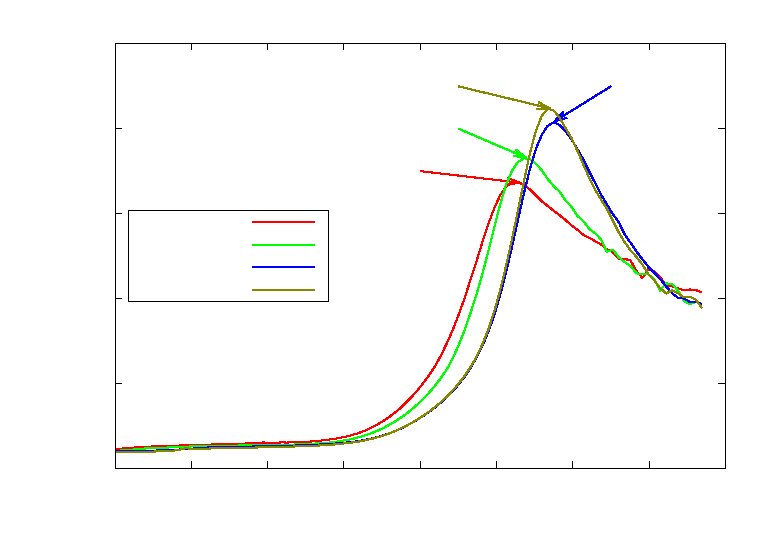
\includegraphics{src/origin/1/tg}}%
    \gplfronttext
  \end{picture}%
\endgroup

    \end{center}
    \caption{外润滑剂玻璃化转变温度}
    \label{fig1Tg}
\end{figure}

根据实验结果,$E_3$ 和 $E_4$ 组具有较高的玻璃化温度,分别为 155.17\cd 和 154.03\cd,比 $E_1$ 和 $E_2$ 组的 146.09\cd 和 147.78\cd 平均高 7\cd 左右。本实验结果与静态热稳定性测试的结果一致,认为玻璃化温度、静态热稳定性与 CPVC 的塑化效果呈正相关。在塑化过程中 AC-316 与 AC-617 对 CPVC 的塑化效果较差,导致体系的受热均匀性也较差。CPVC 分子易发生断裂,或分解脱除 HCl,最终形成分子量较小同时双键较多的分子链。最终 $E_1$ 和 $E_2$ 组的 $T_g$ 较低。

\subsection{本节小结}
本节实验对 AC-316、AC-617、AC-629 和 PEW-0380 四种外润滑剂进行了热性能和力学性能的测试。结果表明,AC-629 与 PEW-0380 外润滑剂为 CPVC 提供较好的润滑效果和塑化效果,使其热稳定性也略好于 AC-316 和 AC-617 组。但由于 AC-617、AC-629 的滴点较低,使其在加工过程中较早失效,使得加工能耗上升。在力学性能的测试中,4 组试样具有相近的拉伸强度与弯曲强度,但 PEW-0380 能使 CPVC 提供最好的冲击强度。因此在加工过程中,若加工温度不高,则外润滑剂可选用润滑效果较好的 AC-629 与 PEW-0380,若加工温度较高,则选用滴点较高的 AC-316 与 PEW-0380。


\section{热稳定体系研究}

\subsection{配方设计}
在本组实验中,我们使用了 TMG-234、T-190A 以及祥生公司的液体有机锡进行测试。有机锡稳定剂的稳定效果较好,可通过特殊的配位作用取代 CPVC 分子上的烯丙基氯原子。但有机锡稳定剂的价格较高,因此我们希望寻找一种在相同用量下稳定效果最好的热稳定剂。因此我们通过控制其他组成不变,单独改变有机锡稳定剂的种类,从而找到一种在相同用量下能实现最好稳定效果且对材料力学性能影响最小的有机锡热稳定剂。具体配方如表 \ref{tab3Pre} 所示。

\begin{table}[!htb]
    \caption{CPVC 3 种有机锡热稳定剂配方设计表}
    \label{tab3Pre}
    \begin{center}
    \footnotesize{
        \begin{tabular}{cccccccccc}
            \borderLine
			组别 & CPVC & \makecell[c]{抗冲击\\改性剂} & \makecell[c]{TMG-\\234} & \makecell[c]{T-\\190A} & \makecell[c]{液体\\有机锡} & 外润滑剂 & 内润滑剂 & 加工助剂 & 钛白粉	\\
            \interLine
            $T_1$ & 100 & 8 & 2 & & & 1.3 & 1.2 & 3 & 2	\\
            $T_2$ & 100 & 8 & & 2 & & 1.3 & 1.2 & 3 & 2	\\
            $T_3$ & 100 & 8 & & & 2 & 1.3 & 1.2 & 3 & 2	\\
            \borderLine
        \end{tabular}
    }
    \end{center}
\end{table}

\subsection{热老化试验箱法}
将 3 组配方的样板进行切割,取 1 $\rm{cm^2}$ 的试样进行测试,结果如表 \ref{tab3static} 所示。

\begin{table}[!htb]
    \caption{$T_1 \sim T_3$ 组热老化试验箱法样品颜色随时间变化}
    \label{tab3static}
    \begin{center}
    \footnotesize{
        \begin{tabular}{cccccccc}
            \borderLine
            \multirow{2}{*}{Sample} & \multicolumn{7}{c}{加入不同种类稳定剂的 CPVC 试样 180\cd 烘箱中颜色随时间的变化}\\
            \cline{2-8}
            & 0 min & 20 min & 30 min & 70 min & 120 min & 250 min & 360 min  \\
            \interLine 
            $T_1$ & \makecell[c]{
\includegraphics[width=.1\linewidth]{src/origin/3/static/00.png}} & \makecell[c]{
\includegraphics[width=.1\linewidth]{src/origin/3/static/01.png}} & \makecell[c]{
\includegraphics[width=.1\linewidth]{src/origin/3/static/02.png}} & \makecell[c]{
\includegraphics[width=.1\linewidth]{src/origin/3/static/03.png}} & \makecell[c]{
\includegraphics[width=.1\linewidth]{src/origin/3/static/04.png}} & \makecell[c]{
\includegraphics[width=.1\linewidth]{src/origin/3/static/05.png}} & \makecell[c]{
\includegraphics[width=.1\linewidth]{src/origin/3/static/06.png}}   \\
            $T_2$ & \makecell[c]{
\includegraphics[width=.1\linewidth]{src/origin/3/static/10.png}} & \makecell[c]{
\includegraphics[width=.1\linewidth]{src/origin/3/static/11.png}} & \makecell[c]{
\includegraphics[width=.1\linewidth]{src/origin/3/static/12.png}} & \makecell[c]{
\includegraphics[width=.1\linewidth]{src/origin/3/static/13.png}} & \makecell[c]{
\includegraphics[width=.1\linewidth]{src/origin/3/static/14.png}} & \makecell[c]{
\includegraphics[width=.1\linewidth]{src/origin/3/static/15.png}} & \makecell[c]{
\includegraphics[width=.1\linewidth]{src/origin/3/static/16.png}}  \\
            $T_3$ & \makecell[c]{
\includegraphics[width=.1\linewidth]{src/origin/3/static/20.png}} & \makecell[c]{
\includegraphics[width=.1\linewidth]{src/origin/3/static/21.png}} & \makecell[c]{
\includegraphics[width=.1\linewidth]{src/origin/3/static/22.png}} & \makecell[c]{
\includegraphics[width=.1\linewidth]{src/origin/3/static/23.png}} & \makecell[c]{
\includegraphics[width=.1\linewidth]{src/origin/3/static/24.png}} & \makecell[c]{
\includegraphics[width=.1\linewidth]{src/origin/3/static/25.png}} & \makecell[c]{\includegraphics[width=.1\linewidth]{src/origin/3/static/26.png}}  \\
            \borderLine
        \end{tabular}
    }
    \end{center}
\end{table}

从表 \ref{tab3static} 可以看出,$T_1$ 和 $T_2$ 组在静态热稳定性上相近,其在 120 min 之前只是轻微变色,在 360 min 时,$T_1$ 和 $T_2$ 组试样明显变黑但未出现明显气泡,此时 CPVC 发生部分分解,分子中产生双键从而发生氧化变黑,但产生的 HCl 量不足以使试样表面产生气泡,可认为加入 TMG-234 和 T-190A 有机锡的试样热稳定性较好,并且可在 190\cd 下维持较长时间的稳定作用。$T_3$ 组在 120 min 前未出现明显变色,甚至略好于 $T_1$ 和 $T_2$ 组的试样,但从 250 min 分钟开始试样表面出现大量气泡,360 min 时试样严重变黑且表面出现大量瘤状气泡。在较短时间内,液体有机锡与 TMG-234、T-190A 的热稳定效果相近,甚至略好。而在较长时间范围内,TMG-234 和 T-190A 的效果明显优于液体有机锡。本实验也从侧面验证了 CPVC 脱 HCl 的链锁分解机理,当 CPVC 分解产生少量 HCl 后,HCl 的分解量会呈几何增长。

\subsection{动态热稳定性测试}
图 \ref{fig3Hakee} 所示为 $T_1 \sim T_3$ 四种配方在转矩流变仪中进行加热剪切过程的 转矩-时间 曲线。由图中数据可得到该体系的熔化转矩、平衡转矩与热稳定时间,具体数据见表 \ref{tab3Hakee}所示。

\begin{figure}[!htb]
    \begin{center}
        % GNUPLOT: LaTeX picture with Postscript
\begingroup
  \makeatletter
  \providecommand\color[2][]{%
    \GenericError{(gnuplot) \space\space\space\@spaces}{%
      Package color not loaded in conjunction with
      terminal option `colourtext'%
    }{See the gnuplot documentation for explanation.%
    }{Either use 'blacktext' in gnuplot or load the package
      color.sty in LaTeX.}%
    \renewcommand\color[2][]{}%
  }%
  \providecommand\includegraphics[2][]{%
    \GenericError{(gnuplot) \space\space\space\@spaces}{%
      Package graphicx or graphics not loaded%
    }{See the gnuplot documentation for explanation.%
    }{The gnuplot epslatex terminal needs graphicx.sty or graphics.sty.}%
    \renewcommand\includegraphics[2][]{}%
  }%
  \providecommand\rotatebox[2]{#2}%
  \@ifundefined{ifGPcolor}{%
    \newif\ifGPcolor
    \GPcolorfalse
  }{}%
  \@ifundefined{ifGPblacktext}{%
    \newif\ifGPblacktext
    \GPblacktexttrue
  }{}%
  % define a \g@addto@macro without @ in the name:
  \let\gplgaddtomacro\g@addto@macro
  % define empty templates for all commands taking text:
  \gdef\gplbacktext{}%
  \gdef\gplfronttext{}%
  \makeatother
  \ifGPblacktext
    % no textcolor at all
    \def\colorrgb#1{}%
    \def\colorgray#1{}%
  \else
    % gray or color?
    \ifGPcolor
      \def\colorrgb#1{\color[rgb]{#1}}%
      \def\colorgray#1{\color[gray]{#1}}%
      \expandafter\def\csname LTw\endcsname{\color{white}}%
      \expandafter\def\csname LTb\endcsname{\color{black}}%
      \expandafter\def\csname LTa\endcsname{\color{black}}%
      \expandafter\def\csname LT0\endcsname{\color[rgb]{1,0,0}}%
      \expandafter\def\csname LT1\endcsname{\color[rgb]{0,1,0}}%
      \expandafter\def\csname LT2\endcsname{\color[rgb]{0,0,1}}%
      \expandafter\def\csname LT3\endcsname{\color[rgb]{1,0,1}}%
      \expandafter\def\csname LT4\endcsname{\color[rgb]{0,1,1}}%
      \expandafter\def\csname LT5\endcsname{\color[rgb]{1,1,0}}%
      \expandafter\def\csname LT6\endcsname{\color[rgb]{0,0,0}}%
      \expandafter\def\csname LT7\endcsname{\color[rgb]{1,0.3,0}}%
      \expandafter\def\csname LT8\endcsname{\color[rgb]{0.5,0.5,0.5}}%
    \else
      % gray
      \def\colorrgb#1{\color{black}}%
      \def\colorgray#1{\color[gray]{#1}}%
      \expandafter\def\csname LTw\endcsname{\color{white}}%
      \expandafter\def\csname LTb\endcsname{\color{black}}%
      \expandafter\def\csname LTa\endcsname{\color{black}}%
      \expandafter\def\csname LT0\endcsname{\color{black}}%
      \expandafter\def\csname LT1\endcsname{\color{black}}%
      \expandafter\def\csname LT2\endcsname{\color{black}}%
      \expandafter\def\csname LT3\endcsname{\color{black}}%
      \expandafter\def\csname LT4\endcsname{\color{black}}%
      \expandafter\def\csname LT5\endcsname{\color{black}}%
      \expandafter\def\csname LT6\endcsname{\color{black}}%
      \expandafter\def\csname LT7\endcsname{\color{black}}%
      \expandafter\def\csname LT8\endcsname{\color{black}}%
    \fi
  \fi
    \setlength{\unitlength}{0.0500bp}%
    \ifx\gptboxheight\undefined%
      \newlength{\gptboxheight}%
      \newlength{\gptboxwidth}%
      \newsavebox{\gptboxtext}%
    \fi%
    \setlength{\fboxrule}{0.5pt}%
    \setlength{\fboxsep}{1pt}%
\begin{picture}(7200.00,5040.00)%
    \gplgaddtomacro\gplbacktext{%
      \csname LTb\endcsname%
      \put(682,704){\makebox(0,0)[r]{\strut{}$0$}}%
      \put(682,1722){\makebox(0,0)[r]{\strut{}$5$}}%
      \put(682,2740){\makebox(0,0)[r]{\strut{}$10$}}%
      \put(682,3757){\makebox(0,0)[r]{\strut{}$15$}}%
      \put(682,4775){\makebox(0,0)[r]{\strut{}$20$}}%
      \put(814,484){\makebox(0,0){\strut{}$0$}}%
      \put(1903,484){\makebox(0,0){\strut{}$2$}}%
      \put(2992,484){\makebox(0,0){\strut{}$4$}}%
      \put(4081,484){\makebox(0,0){\strut{}$6$}}%
      \put(5170,484){\makebox(0,0){\strut{}$8$}}%
      \put(6259,484){\makebox(0,0){\strut{}$10$}}%
    }%
    \gplgaddtomacro\gplfronttext{%
      \csname LTb\endcsname%
      \put(176,2739){\rotatebox{-270}{\makebox(0,0){\strut{}转矩/N$\cdot$m}}}%
      \put(3808,154){\makebox(0,0){\strut{}时间/min}}%
      \csname LTb\endcsname%
      \put(5816,1317){\makebox(0,0)[r]{\strut{}TMG-234}}%
      \csname LTb\endcsname%
      \put(5816,1097){\makebox(0,0)[r]{\strut{}T-190 A}}%
      \csname LTb\endcsname%
      \put(5816,877){\makebox(0,0)[r]{\strut{}Orgin Tin(l)}}%
    }%
    \gplbacktext
    \put(0,0){\includegraphics{src/origin/3/hakee}}%
    \gplfronttext
  \end{picture}%
\endgroup

    \end{center}
    \caption{$T_1 \sim T_3$ 组转矩流变仪 转矩-时间 曲线}
	\label{fig3Hakee}
\end{figure}

\begin{table}[!htb]
    \caption{$T_1 \sim T_3$ 组动态热稳定性能数据表}
    \label{tab3Hakee}
    \begin{center}
    \footnotesize{
        \begin{tabular}{ccccc}
            \borderLine
            组别 & 热稳定剂 & \makecell[c]{熔化转矩 $M_{fus}$/\\N$\cdot$m} & \makecell[c]{平衡转矩$M_{melt}$/\\N$\cdot$m} & \makecell[c]{热稳定时间$T_{s}$/\\min} \\
            \interLine
            $T_1$ & TMG-234 & 19.8 & 10.8 & 6.5	\\
            $T_2$ & T-190A & 19.1 & 10.3 & 6.1	\\
            $T_3$ & 液体有机锡 & 18.8 & 10.1 & 5.4  \\
            \borderLine
        \end{tabular}
    }
    \end{center}
\end{table}

结合图表数据,我们可以看出 $T_1$ 组的熔化转矩略大于 $T_2$ 组和 $T_3$ 组,同时三组的平衡转矩呈 $M_{melt, T_1} > M_{melt, T_2} > M_{melt, T_3}$ 的趋势,三组的热稳定时间也呈 $T_{s, T_1} > T_{s, T_2} > T_{s, T_3}$ 趋势排列。该组的 平衡转矩与热稳定时间呈较好的正相关性,猜测是在 CPVC 发生大量分解之前,液体有机锡的稳定效果较 TMG-234 和 T-190A 略好,但其长期热稳定性较差,导致体系提前进入热分解阶段。

\subsection{力学性能测试}
采用万能试验机对 $T_1 \sim T_3$ 组的标准试样进行拉伸强度、弯曲强度和缺口冲击强度的测试,具体数据如表 \ref{tab3Mach} 所示。

\begin{table}[!htb]
    \caption{$T_1 \sim T_3$ 组力学性能数据表}
    \label{tab3Mach}
    \begin{center}
    \footnotesize{
        \begin{tabular}{ccccc}
			\borderLine
			组别 & \makecell[c]{拉伸强度$\sigma_t$/\\MPa} & \makecell[c]{弯曲强度$\sigma_{b}$/\\Mpa} & \makecell[c]{缺口冲击强度$aiN$/\\$\rm{KJ/m^2}$} & \makecell[c]{断裂伸长率\\\%}	\\
			\interLine
			$T_1$ & 48.84 & 57.40 & 3.50 & 50.45	\\
			$T_2$ & 53.66 & 61.22 & 5.22 & 62.36	\\
			$T_3$ & 54.10 & 59.21 & 7.95 & 81.36	\\
			\borderLine
        \end{tabular}
    }
    \end{center}
\end{table}

由表 \ref{tab3Mach} 中数据,发现对于拉伸强度、缺口冲击强度、断裂伸长率同样呈现了非常好的正相关性,$T_3$ 组的力学性能参数明显优于 $T_1$ 组和 $T_2$ 组。可以推测,我们在实际的 CPVC 塑化以及压片过程中,塑化时间并未达到液体有机锡的热稳定时间上限,此时液体有机锡的热稳定效果是优于 TMG-234 和 T-190A 的,其在不影响 CPVC 树脂热稳定性的情况下还能提供较好的塑化效果,使得 $T_3$ 组的拉伸强度、缺口冲击强度和断裂伸长率的损失较小。

\subsection{动态力学热分析(DMA)}
根据 $T_1 \sim T_3$ 三组配方的 损耗因子-时间 数据制得图 \ref{fig3Tg},取损耗因子的峰值温度作为试样的玻璃化转变温度。

\begin{figure}[!htb]
    \begin{center}
        % GNUPLOT: LaTeX picture with Postscript
\begingroup
  \makeatletter
  \providecommand\color[2][]{%
    \GenericError{(gnuplot) \space\space\space\@spaces}{%
      Package color not loaded in conjunction with
      terminal option `colourtext'%
    }{See the gnuplot documentation for explanation.%
    }{Either use 'blacktext' in gnuplot or load the package
      color.sty in LaTeX.}%
    \renewcommand\color[2][]{}%
  }%
  \providecommand\includegraphics[2][]{%
    \GenericError{(gnuplot) \space\space\space\@spaces}{%
      Package graphicx or graphics not loaded%
    }{See the gnuplot documentation for explanation.%
    }{The gnuplot epslatex terminal needs graphicx.sty or graphics.sty.}%
    \renewcommand\includegraphics[2][]{}%
  }%
  \providecommand\rotatebox[2]{#2}%
  \@ifundefined{ifGPcolor}{%
    \newif\ifGPcolor
    \GPcolorfalse
  }{}%
  \@ifundefined{ifGPblacktext}{%
    \newif\ifGPblacktext
    \GPblacktexttrue
  }{}%
  % define a \g@addto@macro without @ in the name:
  \let\gplgaddtomacro\g@addto@macro
  % define empty templates for all commands taking text:
  \gdef\gplbacktext{}%
  \gdef\gplfronttext{}%
  \makeatother
  \ifGPblacktext
    % no textcolor at all
    \def\colorrgb#1{}%
    \def\colorgray#1{}%
  \else
    % gray or color?
    \ifGPcolor
      \def\colorrgb#1{\color[rgb]{#1}}%
      \def\colorgray#1{\color[gray]{#1}}%
      \expandafter\def\csname LTw\endcsname{\color{white}}%
      \expandafter\def\csname LTb\endcsname{\color{black}}%
      \expandafter\def\csname LTa\endcsname{\color{black}}%
      \expandafter\def\csname LT0\endcsname{\color[rgb]{1,0,0}}%
      \expandafter\def\csname LT1\endcsname{\color[rgb]{0,1,0}}%
      \expandafter\def\csname LT2\endcsname{\color[rgb]{0,0,1}}%
      \expandafter\def\csname LT3\endcsname{\color[rgb]{1,0,1}}%
      \expandafter\def\csname LT4\endcsname{\color[rgb]{0,1,1}}%
      \expandafter\def\csname LT5\endcsname{\color[rgb]{1,1,0}}%
      \expandafter\def\csname LT6\endcsname{\color[rgb]{0,0,0}}%
      \expandafter\def\csname LT7\endcsname{\color[rgb]{1,0.3,0}}%
      \expandafter\def\csname LT8\endcsname{\color[rgb]{0.5,0.5,0.5}}%
    \else
      % gray
      \def\colorrgb#1{\color{black}}%
      \def\colorgray#1{\color[gray]{#1}}%
      \expandafter\def\csname LTw\endcsname{\color{white}}%
      \expandafter\def\csname LTb\endcsname{\color{black}}%
      \expandafter\def\csname LTa\endcsname{\color{black}}%
      \expandafter\def\csname LT0\endcsname{\color{black}}%
      \expandafter\def\csname LT1\endcsname{\color{black}}%
      \expandafter\def\csname LT2\endcsname{\color{black}}%
      \expandafter\def\csname LT3\endcsname{\color{black}}%
      \expandafter\def\csname LT4\endcsname{\color{black}}%
      \expandafter\def\csname LT5\endcsname{\color{black}}%
      \expandafter\def\csname LT6\endcsname{\color{black}}%
      \expandafter\def\csname LT7\endcsname{\color{black}}%
      \expandafter\def\csname LT8\endcsname{\color{black}}%
    \fi
  \fi
    \setlength{\unitlength}{0.0500bp}%
    \ifx\gptboxheight\undefined%
      \newlength{\gptboxheight}%
      \newlength{\gptboxwidth}%
      \newsavebox{\gptboxtext}%
    \fi%
    \setlength{\fboxrule}{0.5pt}%
    \setlength{\fboxsep}{1pt}%
\begin{picture}(7200.00,5040.00)%
    \gplgaddtomacro\gplbacktext{%
      \csname LTb\endcsname%
      \put(814,704){\makebox(0,0)[r]{\strut{}$0$}}%
      \put(814,1518){\makebox(0,0)[r]{\strut{}$0.2$}}%
      \put(814,2332){\makebox(0,0)[r]{\strut{}$0.4$}}%
      \put(814,3147){\makebox(0,0)[r]{\strut{}$0.6$}}%
      \put(814,3961){\makebox(0,0)[r]{\strut{}$0.8$}}%
      \put(814,4775){\makebox(0,0)[r]{\strut{}$1$}}%
      \put(946,484){\makebox(0,0){\strut{}$40$}}%
      \put(1678,484){\makebox(0,0){\strut{}$60$}}%
      \put(2410,484){\makebox(0,0){\strut{}$80$}}%
      \put(3142,484){\makebox(0,0){\strut{}$100$}}%
      \put(3875,484){\makebox(0,0){\strut{}$120$}}%
      \put(4607,484){\makebox(0,0){\strut{}$140$}}%
      \put(5339,484){\makebox(0,0){\strut{}$160$}}%
      \put(6071,484){\makebox(0,0){\strut{}$180$}}%
      \put(6803,484){\makebox(0,0){\strut{}$200$}}%
    }%
    \gplgaddtomacro\gplfronttext{%
      \csname LTb\endcsname%
      \put(176,2739){\rotatebox{-270}{\makebox(0,0){\strut{}损耗因子}}}%
      \put(3874,154){\makebox(0,0){\strut{}温度/\cd}}%
      \csname LTb\endcsname%
      \put(2662,4602){\makebox(0,0)[r]{\strut{}TMG-234}}%
      \csname LTb\endcsname%
      \put(2662,4382){\makebox(0,0)[r]{\strut{}T-190 A}}%
      \csname LTb\endcsname%
      \put(2662,4162){\makebox(0,0)[r]{\strut{}Orgin Tin(l)}}%
    }%
    \gplbacktext
    \put(0,0){\includegraphics{src/origin/3/tg}}%
    \gplfronttext
  \end{picture}%
\endgroup

    \end{center}
    \caption{热稳定体系玻璃化转变温度}
	\label{fig3Tg}
\end{figure}

分析图 \ref{fig3Tg} 中数据得,$T_2$ 组具有最高的 $T_g$,比 $T_1$ 和 $T_3$ 组平均高了 13.5\cd,可以确定 $T_2$ 组的 CPVC 分子链的刚性较大。

\subsection{维卡软化点}
将 $T_1 \sim T_3$ 组试样置入维卡软化点试验机中进行测试,记录针头压入 1 mm 时的温度如表 \ref{tab3Vic} 所示。

\begin{table}
	\caption{热稳定体系维卡软化点数据表}
	\label{tab3Vic}
	\begin{center}
	\footnotesize{
		\begin{tabular}{p{.2\textwidth}p{.2\textwidth}}
			\borderLine
			\makecell[c]{sample} & \makecell[c]{维卡软化点\\\cd}	\\
			\interLine
			\makecell[c]{$T_1$} & \makecell[c]{114.9}	\\
			\makecell[c]{$T_2$} & \makecell[c]{117.0}	\\
			\makecell[c]{$T_3$} & \makecell[c]{116.4}	\\
			\borderLine
		\end{tabular}
	}
	\end{center}
\end{table}

由表 \ref{tab3Vic} 中数据可见,$T_2$ 组的维卡软化点最高,与动态力学热分析的测试结果一致。因此推测加入 T-190A 可使 CPVC 树脂在高温下仍保持较高的硬度和强度。

\subsection{本节小结}
在本节实验中,我们对 TMG-234、T-190A 和液体有机锡 3 种有机锡热稳定剂进行了热性能与力学性能的测试。实验结果表明,液体有机锡的短期热稳定性略好于 TMG-234 和 T-190A 热稳定剂,但液体有机锡的长期热稳定性较差且热稳定时间短。在塑化时间要求较短的情况下可选用液体有机锡热稳定剂,要求时间较长的情况下需选用 TMG-234、T-190A 热稳定剂。力学性能测试显示,液体有机锡使 CPVC 的强度与韧性的损失较小。同时 T-190A 体系的 $T_g$ 较高,其在较高温度下仍能使 CPVC 提供较高的强度与硬度。